\documentclass{beamer}

\usepackage[utf8]{inputenc}
\usepackage{lmodern}
\inputencoding{utf8}

\usepackage{tikz}
\usepackage{minted} % syntax highlighting
\usetikzlibrary{positioning}
\usepackage{csquotes}

\definecolor{gris}{rgb}{0.92,0.92,0.92}
\definecolor{blau-upc}{rgb}{.192,.365,.506}

\setbeamercolor{titlelike}{fg=blau-upc}
% \setbeamercolor{barra}{bg=white,fg=white}
\setbeamercolor{capcalera}{bg=blau-upc,fg=white}
\setbeamercolor{section in toc}{fg=blau-upc}
\setbeamertemplate{sections/subsections in toc}[circle]
\setbeamertemplate{itemize items}[circle]
\setbeamercolor{item}{fg=blau-upc}
\setbeamertemplate{blocks}[rounded][shadow=true]
\setbeamercolor*{block body}{bg=gris}
\setbeamerfont{block body}{size=\footnotesize}
\setbeamercolor*{block title}{parent=structure,bg=blau-upc,fg=white}

\setbeamersize{text margin left=12mm,text margin right=12mm}
\setbeamertemplate{navigation symbols}{}

\defbeamertemplate*{headline}{infolines theme}
{
	\begin{beamercolorbox}[wd=\paperwidth,ht=9.5mm,right]{white}%
		\includegraphics[height=8mm]{./figures/imperial.pdf}\hspace*{1mm}\vskip0.2ex
	\end{beamercolorbox}
% 	\begin{beamercolorbox}[wd=\paperwidth,ht=0.5mm,left]{barra}%
% 		\hspace*{1mm}
% 	\end{beamercolorbox}
}

\setbeamertemplate{footline}
{
	\hbox{
	\begin{beamercolorbox}[wd=0.1\paperwidth,ht=10mm,left]{}
% 		\hspace*{1ex}\includegraphics[height=8mm]{./logotips/imperiallogo.pdf}\vskip 2ex
	\end{beamercolorbox}
	\begin{beamercolorbox}[wd=0.8\paperwidth,ht=3ex,center]{}
		\hspace*{4ex}\insertsection\vskip 4ex
	\end{beamercolorbox}
	\begin{beamercolorbox}[wd=0.1\paperwidth,ht=3ex,right]{}
		\insertpagenumber\hspace*{6ex}\vskip 4ex
	\end{beamercolorbox}
	}
}

\setbeamertemplate{title page}
{
	\vbox{}
	\vfill
	\begin{centering}
		{\usebeamerfont{title}\usebeamercolor[fg]{title}\inserttitle}
		\vskip0.2em
		{\usebeamerfont{subtitle}\usebeamercolor[fg]{subtitle}\insertsubtitle}
		\vskip2em\par
		\small\insertauthor\par
		\vskip0.7em\par
		\tiny\insertdate\vskip1em\par
	\end{centering}
% 	\vfill
}


%%%%%%%%%%%%%%%%%%%%%%%%%%%%%%%%%%%%%%%%%
% University Assignment Title Page 
% LaTeX Template
% Version 1.0 (27/12/12)
%
% This template has been downloaded from:
% http://www.LaTeXTemplates.com
%
% Original author:
% WikiBooks (http://en.wikibooks.org/wiki/LaTeX/Title_Creation)
%
% License:
% CC BY-NC-SA 3.0 (http://creativecommons.org/licenses/by-nc-sa/3.0/)
% 
%
%%%%%%%%%%%%%%%%%%%%%%%%%%%%%%%%%%%%%%%%%
%----------------------------------------------------------------------------------------
%	PACKAGES AND OTHER DOCUMENT CONFIGURATIONS
%----------------------------------------------------------------------------------------
%\usepackage[a4paper,hmargin=2.8cm,vmargin=2.0cm,includeheadfoot]{geometry}
%\usepackage{textpos}
%\usepackage[backend=bibtex,sorting=none]{biblatex}
%\usepackage{tabularx,longtable,multirow,subfigure,caption}%hangcaption
%\usepackage{fncylab} %formatting of labels
%\usepackage{fancyhdr} % page layout
%\usepackage{url} % URLs
%\usepackage[english]{babel}
%\usepackage{amsmath}
%\usepackage{graphicx}
%\usepackage{dsfont}
%\usepackage{epstopdf} % automatically replace .eps with .pdf in graphics
%\usepackage{array}
%\usepackage{latexsym}
%\usepackage[pdftex,hypertexnames=false,colorlinks]{hyperref} % provide links in pdf

% additional

\usepackage{caption}

%%%%%% TITLE, AUTHOR, DATE DEFINITIONS %%%%%%
\title{Making Smart Contracts Safer}
\author{Aurel Bílý, Catalin Craciun, Calin Farcas,\\Constantin Mueller, Yicheng Luo, Niklas Vangerow}
\date{\today}
%%%%%%

\begin{document}

\begin{frame}
\titlepage
\end{frame}

\begin{frame}
\frametitle{Contents}
\tableofcontents
\end{frame}

% FIRST SIXTY SECONDS
% Smart contracts have the potential to be a hugely disruptive technology. 
% They are decentralised applications that could transform areas such as banking, 
% insurance and even our voting system. 
% At the moment, most smart contracts are written in Solidity, 
% a language with many flaws considering smart contracts need to be very safe. 
% Because of this, Franklin Schrans developed Flint under Susan's supervision. 
% Flint is a programming language for smart contracts aimed to be much safer while being simple to use. 
% However, before our work, Flint was not usable in practice due to a number of bugs and the lack of essential features. 
% For our third-year group project we worked on adding those features and 
% improving the Flint ecosystem to make Flint more useful in the real world.*

% * not actually

\section{Problems with Smart Contracts}
%
% Problem statement
%
% Let's take a step back................
% Ethereum is a distributed application ecosystem on the blockchain.
% Users may execute arbitrary code snippets running on the Ethereum 
% Virtual Machine, EVM for short; these applications are called smart contracts.
% As you can imagine, writing EVM byte-code is not fun, a bit like 
% writing assembly code by hand.
% You might know about the Solidity programming language, which aimed
% to simplify writing smart contracts; it's something like the 
% PHP of smart contract programming languages.
% Flint is an attempt at creating a safer, less error prone programming
% language for Ethereum smart contract development. The underpinning 
% philosophy is simplicity, and its design has been largely inspired by
% the Swift programming language. Creating a safe language involves 
% prohibiting many avoidable programmer errors at compile-time. At the
% moment, these avoidable errors put hundreds of millions of dollars
% worth of cryptocurrencies at risk.
%

\begin{frame}
\frametitle{Motivation}
\begin{itemize}
    \item Writing smart contracts is currently only possible with Solidity, or EVM.
\end{itemize}
\end{frame}

\section{Problems with Flint}
% As mentioned before, as of October there were still serious flaws in Flint.
% In particular, Flint does not allow for external calls, i.e. function calls to
% other contracts, which are an absolute necessity to process currency.
% In plain words, Flint cannot be used to develop smart contracts without external calls.
% In addition, Flint - like Solidity - used to treat Ether as integers which 
% could easily to "losing" currency. Remember that a contract is entirely controlled
% by its code and that the code is immutable.
% Also, Flint had no real ecosystem for development and no testing, meaning that there
% were plenty of additions and improvements for us to make.

\section{Achievements}
\subsection{Asset Traits with Self}

\begin{frame}{What are Asset Traits?}
% Think of a Flint trait like a Java interface.
% The purpose of adding an asset trait is to reduce duplication when defining
%   assets, such as Wei. Reducing duplication prevents a programmer from forgetting
%   to implement safety precautions necessary for functions such as `transfer`
\end{frame}

\begin{frame}{Cross-Asset Transfers}
% One thing that we want to prevent is one asset being transferred to another
% This can be done with a polymorphic self type or generics. 
% We chose not to implement generics due to our time on the project being limited o
% and them being complex, going against the language principle of simplicity.
\end{frame}

\begin{frame}{Polymorphic Self}
% Rather than implementing generics in the language, we implemented a 
% polymorphic self type.
% As you can see, Self is treated as the implementing type at the calling site,
% but functions in place of the trait in the context of the trait.
% example of type signatures
\end{frame}

\begin{frame}{Creating an Asset}
% a code example of how an Asset is implemented
\end{frame}

\subsection{Unit Testing}
\begin{frame}{Why Test?}
% After working on the compiler for a few weeks, it became increasingly clear
% that many of the features that we had assumed were implemented, were only
% implemented partially.
% Due to a lack of unit tests, we had no way to know whether our features
% worked in isolation, whether there were any regressions
% We also had to verify that our new additions worked by testing manually
\end{frame}
% After working for a few weeks, it became increasingly clear that the lack of proper unit testing was becoming very problematic, since we only had few signals of feature regression. While some tests already existed, they were rather ad-hoc and focused on the overall behaviour of the compiler; there was no unit testing or mocking to allow us to test smaller components in isolation, which would make it easier to track down the source of a problem.
% 
% Setting up testing was a major challenge as Swift is a new language. From the start we wanted to have the ability to mock and stub protocols and classes to write effective unit tests but we found that there were several problems with this: First, Swift has very limited reflection capabilities. Reflection in Swift is read-only, which means that any kind of run-time stubbing like done in JMock\footnote{\url{http://jmock.org/}} and other Java testing frameworks is impossible. Second, the ecosystem is not yet very mature. Swift frameworks are often created by independent developers as industry adoption has been fairly slow. There are several testing frameworks on the Internet but all of them suffer from lack of maintenance, often being outdated and incompatible with Swift 4.2, the version of Swift that we are targeting.
% 
% Overcoming the reflection issue meant taking an approach that is applied in other languages, such as Go, that lack powerful reflection capabilities, which is static code generation. Essentially, we create stubs and mocks for all of our protocols and classes ahead of time by analysing the source code, and compile these into our unit testing target. To enable mocks to be used in place of concrete implementations, Swift forces us to use protocols or classes as structures cannot be subclassed.
% 
% Implementing this type of code generation from scratch is a significant time investment. In our search we had attempted to integrate several different frameworks, including SwiftMock\footnote{\url{https://github.com/mflint/SwiftMock}} and had even considered to write the code generation or boilerplate ourselves. After many hours of searching, we found a framework called Cuckoo\footnote{\url{https://github.com/Brightify/Cuckoo} and our fork \url{https://github.com/flintrocks/Cuckoo}} which met all of the requirements that we had:
% 
% Easy integration: We want the framework to be easy to integrate into the project and into an existing codebase with minimal code changes required.
% Low boilerplating: We wish to automate the majority (or all) of the workflow.
% Easy-to-use API: Writing tests should be familiar and intuitive, an API for mock specification and verification should be similar to other established frameworks in the industry.
% 
% Integrating Cuckoo proved to be a challenging task. Cuckoo was not updated for the version of Swift we were targeting, and wholly incompatible with Linux. Since our development environments were cross-platform and our continuous integration ran on Linux, we needed to keep our codebase compatible with both macOS and Linux. As a result, we made a fork of Cuckoo and its dependencies and slowly updated them to work on Swift 4.2 as well as on Linux. In the long term this means that there are additional frameworks to maintain, but the hope is that the changes that we have made can either be contributed back to the original projects or that the maintainers find some time and make their own modifications to allow Swift 4.2 and Linux compatibility.
% 
% Once we had set up mocking, we had to choose a unit testing framework. We chose XCTest as it is supported by Apple and integrated into both the Swift package manager, which is used to compile the project and its dependencies, and Xcode. The Flint compiler is organised into several `modules' that allow us to use and re-use different parts of the compiler for a set of targets (tests, flintc, IDE integration, etc). With XCTest we were able to create test targets that correspond to these modules and contain tests that test code defined within those modules. Our Makefile allows us to compile all mocks and stubs prior to building the test targets themselves to guarantee that their interfaces are up to date.
% 
% Writing tests is a major undertaking and should ideally have been done from the start of the project. As we did not have much time to execute a major refactoring of the codebase to make testing easier, we decided to focus on a select few units and wrote several tests for these to demonstrate how a test can be written. Writing tests retroactively requires an intricate knowledge of the functionality and specification of each unit, but in the future, further tests need to be written to increase the code coverage. In some of our work following the availability of testing in the project, we opted to use a Test Driven Development (TDD) workflow to test our assumptions and specify our code well. Below is an example of a unit test, showing the environment of an ASTPassContext stubbed with a faux testing response.

\subsection{General Improvements}

\begin{frame}
% We have also implemented/fixed/improved a number of smaller features, many of which were found while trying to solve different problems.
\frametitle{General Improvements}
\begin{itemize}
    \item Right associativity of the dot operator
    \item Unification of event and function declaration syntax
    \item Function calls parameter passing/ordering
\end{itemize}
\end{frame}

\begin{frame}
% Due to the nature of the parser, the dot operator was right associative, making it completely impractical to access nested fields of a struct. This was fixed by performing rotations for the dot operator after parsing. 
\frametitle{Right associativity of the dot operator}
\begin{itemize}
    \item a.(b.(c.d)) vs ((a.b).c).d
\end{itemize}
\end{frame}

\begin{frame}
% Unified the declaration syntax for events and functions to increase clarity.
\frametitle{Events and functions}
\begin{itemize}
    \item Unify the declaration syntax
    \item Implement default parameters for functions (previously only for events - not working)
\end{itemize}
\end{frame}

\begin{frame}
% Unified the declaration syntax for events and functions to increase clarity.
\frametitle{Function Call Parameters}
\begin{itemize}
    \item New logic for parameter checking (includes default parameters)
    \item Enforce labels and Swift-like ordering
\end{itemize}
\end{frame}

% These feed into the Demo
\subsection{Language Server Protocol}
\subsection{External Calls with Error Handling}
\section{Demo}

\section{Extensions}
% Linear types are a more integrated version of the Asset traits that we have implemented. These types might be implemented with additional syntax and memory operations, allowing variables that hold quantities of an asset that can be split atomically, never duplicated, and never destroyed\cite{flint-paper}. For example, with an asset such as Wei in the context of a @payable contract function, this means we add a semantic check that ensures that the entire value of the incoming asset value is transferred to another instance to prevent its destruction.
\subsection{Linear Types}

\begin{frame}
\frametitle{Linear Types}
\begin{itemize}
    \item Treating assets as integer values is a source of numerous bugs and exploits not only on the Ethereum network
    \item Linear types would be integrated into the language to never allow an asset to be destroyed, duplicated, or created from scratch
\end{itemize}
\end{frame}

\begin{frame}
\frametitle{Linear Types Example}
\inputminted{swift}{code/linear-types.flint}
\end{frame}

% Adding modules allows a contract definition to be split across multiple source files and for the inclusion and distribution of user-made libraries and frameworks.
\subsection{Modularisation}

% A package manager has long been a requested feature, but until we implemented external calls there was no reason to have one because there would've been no way to call another contract. Additionally, since the language does not currently support modules, there is no way to import code from another Flint program. Once modules and a Flint ABI are supported, there will be a better case for having a package manager.
\subsection{Package Manager}

\begin{frame}
 	\vbox{}
% 	\vfill
	\begin{centering}
	{\LARGE \usebeamercolor[fg]{title} Thanks for watching, please commend and subscribe and SMASH that mf like button}
	\par
	\end{centering}
\end{frame}
%﷽﷽ FIN ﷽﷽
%﷽﷽ FIN ﷽﷽
%﷽﷽ FIN ﷽﷽
%﷽﷽ FIN ﷽﷽

\begin{frame}
\frametitle{Example Contract}
\inputminted[fontsize=\tiny]{swift}{code/wallet.flint}
\end{frame}

\begin{frame}{Codebase}
\begin{figure}[htbp]
\centering
\resizebox {\columnwidth} {!} {
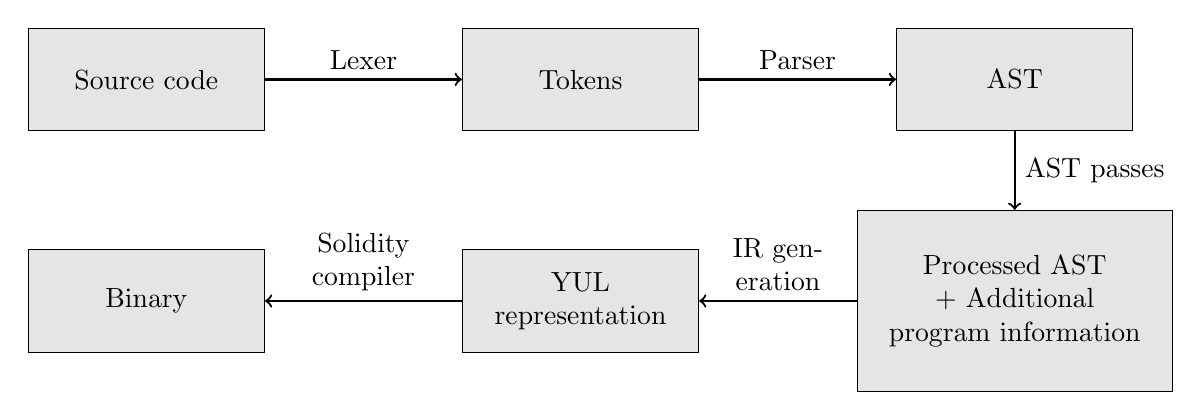
\begin{tikzpicture}[%
	main node/.style={
		rectangle,
		fill=gray!20,
		draw,
		minimum width=3cm,
		minimum height=1.3cm,
		inner sep=0pt,
		%text height=1.5ex,
		text width=3cm,
		%text depth=.25ex,
		align=center
	},
	large node/.style={
		rectangle,
		fill=gray!20,
		draw,
		minimum width=4cm,
		minimum height=2.3cm,
		inner sep=0pt,
		%text height=1.5ex,
		text width=4cm,
		%text depth=.25ex,
		align=center
	},
]
	\node[main node] (1) {Source code};
	\node[main node] (2) [right = 2.5cm of 1] {Tokens};
	\node[main node] (3) [right = 2.5cm of 2] {AST};
	\node[large node] (4) [below = 1cm of 3] {Processed AST \\ + Additional \\ program information};
	\node[main node] (5) [left = 2cm of 4] {YUL \\ representation};
	\node[main node] (6) [left = 2.5cm of 5] {Binary};
	\path[draw,thick,->]
	(1) edge node [above] {Lexer} (2)
	(2) edge node [above] {Parser} (3)
	(3) edge node [right] {AST passes} (4)
	(4) edge node [above,text width=1.9cm,align=center] {IR generation} (5)
	(5) edge node [above,text width=1.9cm,align=center] {Solidity compiler} (6);
\end{tikzpicture}
}
\caption{Graphic representation of the Flint compilation process.}
\label{flint-compilation}
\end{figure}

\end{frame}

\begin{frame}
\frametitle{Wei}
\end{frame}

\begin{frame}
\frametitle{Addresses and Callers}
\end{frame}


\begin{frame}{Flint: Before and After}
\begin{columns}
    \begin{column}{0.5\textwidth}
        \includegraphics[scale=0.5]{figures/flint-fire.jpg}
    \end{column}
    \begin{column}{0.5\textwidth}
        \includegraphics[scale=0.2]{figures/flint-after.jpg}
    \end{column}
\end{columns}
\end{frame}

\begin{frame}
\frametitle{Programming Languages for Smart Contracts}
\begin{columns}
\begin{column}{0.33\textwidth}
    \begin{block}{EVM}
    	\begin{itemize}
        \item Assembly for Ethereum
        \item Powerful but cumbersome, not safe.
        \end{itemize}
    \end{block}
\end{column}
\begin{column}{0.33\textwidth}
    \begin{block}{Solidity}
        \begin{itemize}
        \item PHP for Ethereum
        \item Not safe
        \end{itemize}
    \end{block}
\end{column}
\begin{column}{0.33\textwidth}
    \begin{block}{Flint}
    \begin{itemize}
    \item Safe
    \item Safe
    \item Safe
    \end{itemize}
    \end{block}
\end{column}

\end{columns}
\end{frame}

\begin{frame}
\frametitle{Language features}
\begin{itemize}
	\item Asset trait
	\item External calls
	\item Better testing
	\item Refactored code generation
	\item General declarations
\end{itemize}
\end{frame}

\begin{frame}\frametitle{Asset traits}
\begin{columns}
\begin{column}{0.5\textwidth}
	\inputminted[fontsize=\tiny]{swift}{code/asset-traits-before.flint}
	Before
\end{column}
\begin{column}{0.5\textwidth}
	\inputminted[fontsize=\tiny]{swift}{code/asset-traits-after.flint}
	After
\end{column}
\end{columns}
\end{frame}

\begin{frame}
\frametitle{External calls - Modes}
\inputminted[fontsize=\small]{swift}{code/modes.flint}
\end{frame}

\frame{\frametitle{Complete example - Weather station}
}

% We also improved the code generation phase of the Flint compiler, which enables us to implement code generation for exception handling and improves the extensibility of the code generator.

% Prior to our refactor, the code generator was architected around simple string concatenation. This was useful as a first prototype, demonstrating that IR conforming to the YUL specification can be generated successfully. However, the implementation introduced complications that prohibited further extension and improvement, such as making it impossible to get a reference to the result of an expression.

% With the initial implementation, it was impossible to generate code for external calls since we needed to store the success status of external calls, in addition to value returned. Our very first attempt at the refactoring creates function signature in the for for of f -> (preamble, expression) where the preamble represented ‘setup’ code and the expression was simply an identifier pointing to the result of evaluating the code. However, there is a lot of preamble to keep track of.

% Lack of jump makes codegen for do-catch difficult. This requires backtracking of the most recent outer do-catch block. We use a stack to keep track of that.

% ```duplication is far cheaper than the wrong abstraction'''

% We make the codegen more sophisticated by introducing types for YUL IR. This is
% code gen done right.
% Another software engineering group worked on improving the YUL IR and implementing a new compiler for YUL. Their implementation might introduce useful extensions to YUL. With this refined design, we can easily extend our YUL definitions and utilise these new extensions.


\begin{frame}
\frametitle{Code generator}
\inputminted[fontsize=\tiny]{swift}{code/codegen.flint}
\end{frame}

\begin{frame}
\frametitle{Toolchain}
\begin{block}{IDE Integration}
	{\tiny
	\begin{itemize}
		\item Language Server/Client (LSP)
	\end{itemize}
	}
\end{block}
\end{frame}

\begin{frame}
\frametitle{Toolchain}
\begin{figure}
    \centering
    \includegraphics[width=0.6\textwidth]{figures/lsp-use.png}
    \\ LSP client running in VSCode
    \label{fig:my_label}
\end{figure}
\end{frame}

\end{document}